Number of features for \Nystrom: $1250, 2500, 5000, 10000, 20000$

Number of features for RFF related approach: $1250, 2500, 5000, 10000, 20000, 50000, 100000, 200000, 400000$


Learning rate search grid for different dataset: 

\begin{table}
	\centering
	\begin{tabular}{c | c | c}
	\hline
	Dataset & $1/2\sigma^2$ & Learning rate grid \\
	\hline
	\hline
Census & 0.0006 & {0.01, 0.05, 0.1, \textbf{0.5}, 1.0} \\
YearPred & 0.01 & {0.05, 0.1, \textbf{0.5}, 1.0, 5.0} \\
Covtype & 0.6 & {1.0, 5.0, 10.0, \textbf{50.0}, 100.0} \\
TIMIT & 0.0015 & {5.0, 10.0, 50.0, \textbf{100.0}, 500.0} \\
	\hline
	\end{tabular}
	\caption{The configuration for Gaussian kernel and the search grid for initial learning rate on the Census, YearPred, Covtype and TIMIT datasets.}
	\label{tab:hyperparam}
\end{table}

\begin{table}
\centering
	\begin{tabular}{c | c | c | c | c }
	\hline
		Dataset & Task & \# train samples & \# heldout samples & \# raw features \\
	\hline
	\hline
		Census & & & & \\
		YearPred & & & & \\
		Covtype & & & &\\
		TIMIT & & & & \\
	\hline
	\end{tabular}
	\caption{Details on the Census, YearPred, Covtype and TIMIT datasets.}
	\label{tab:datasets}
\end{table}


\begin{figure}
	\centering
	\begin{tabular}{c@{\hskip 0in}c@{\hskip 0in}c@{\hskip 0in}c}
		\subfigure[Census heldout MSE]{\label{fig:census_mem} 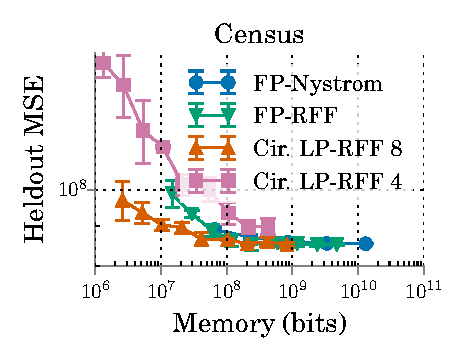
\includegraphics[width=0.3\linewidth]{figures/census_MSE_vs_n_memory.pdf} } \hfill
		\subfigure[Census heldout MSE]{\label{fig:census_feat}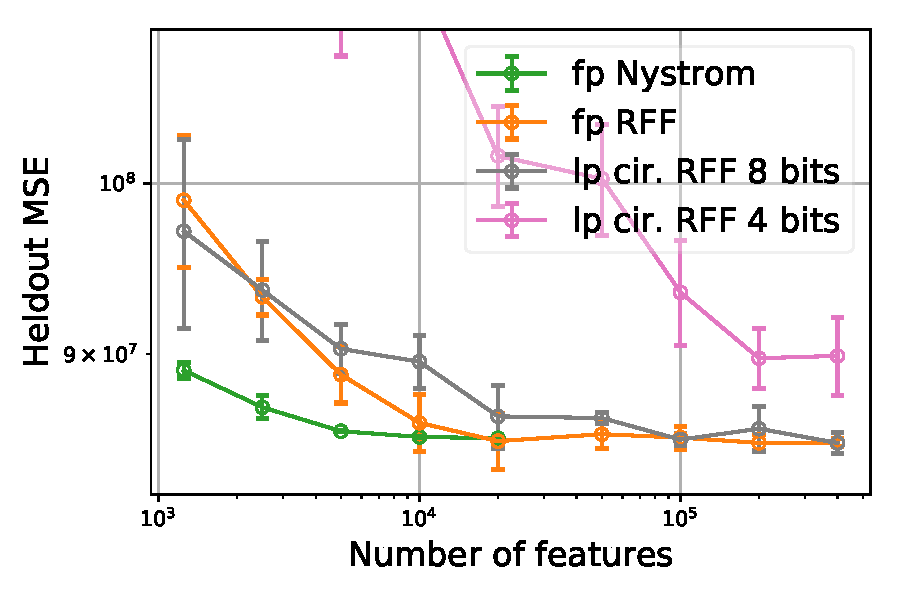
\includegraphics[width=0.3\linewidth]{figures/census_MSE_vs_n_feat.pdf} } \hfill
		\subfigure[CovType heldout error]{\label{fig:covtype_mem} 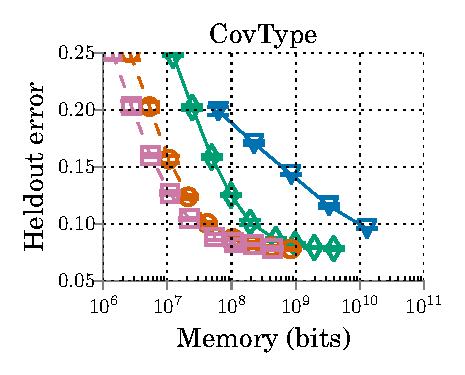
\includegraphics[width=0.3\linewidth]{figures/covtype_error_vs_n_memory.pdf} } \hfill
		\subfigure[CovType heldout error]{\label{fig:covtype_feat}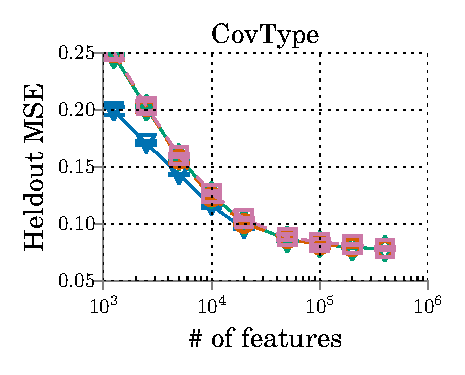
\includegraphics[width=0.3\linewidth]{figures/covtype_error_vs_n_feat.pdf} } \hfill
%		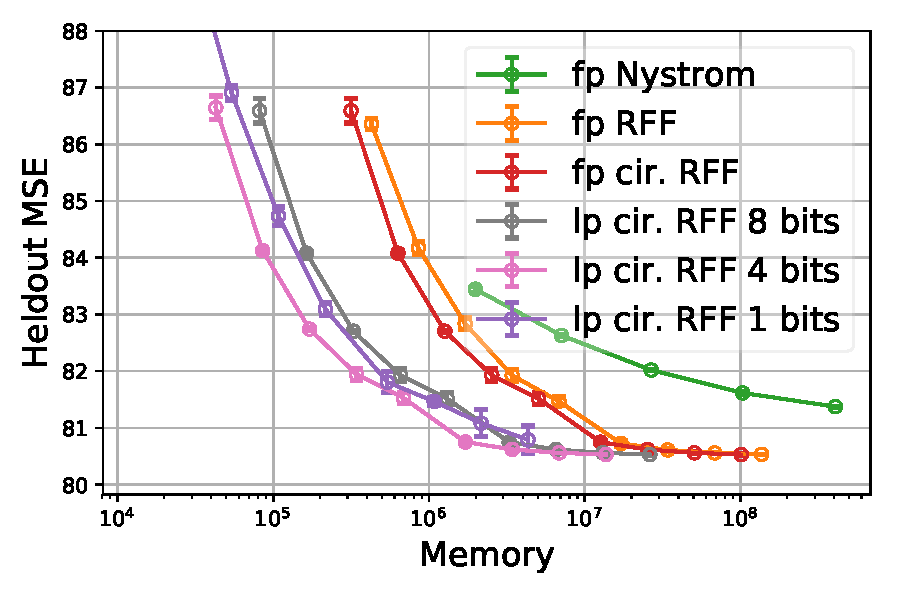
\includegraphics[width=0.3\linewidth]{figures/yearpred_MSE_vs_n_memory.pdf} &
%		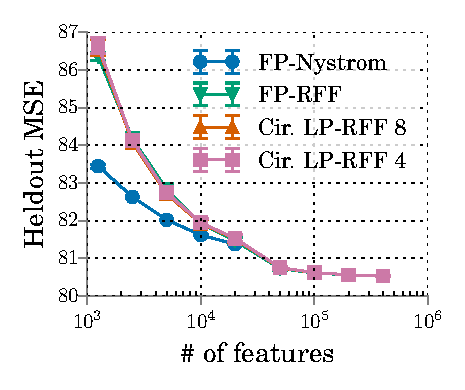
\includegraphics[width=0.3\linewidth]{figures/yearpred_MSE_vs_n_feat.pdf} &
%		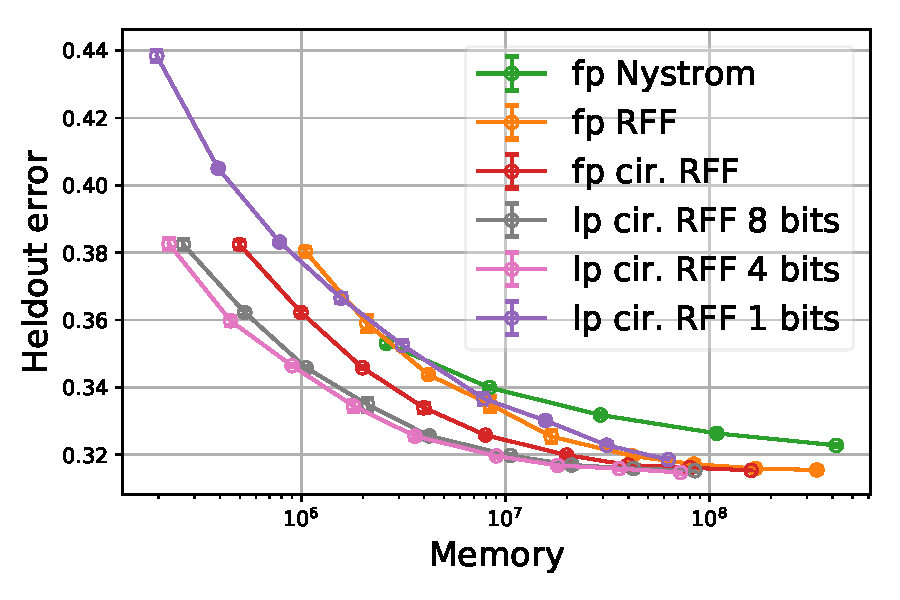
\includegraphics[width=0.3\linewidth]{figures/timit_error_vs_n_memory.pdf} &
%		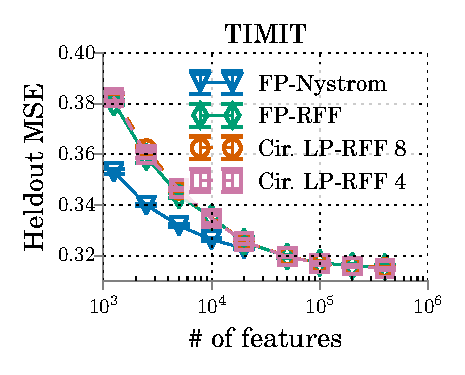
\includegraphics[width=0.3\linewidth]{figures/timit_error_vs_n_feat.pdf} \\
%		(a) Census & (b) YearPred & (c) Covtype & (d) TIMIT \\
%		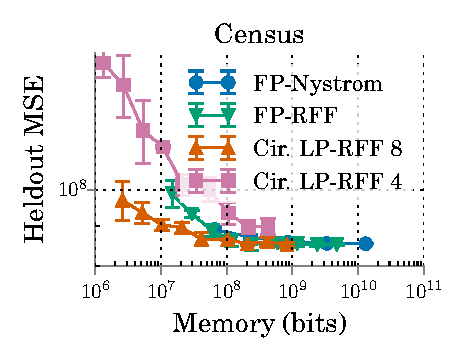
\includegraphics[width=0.3\linewidth]{figures/census_MSE_vs_n_memory.pdf} &
%		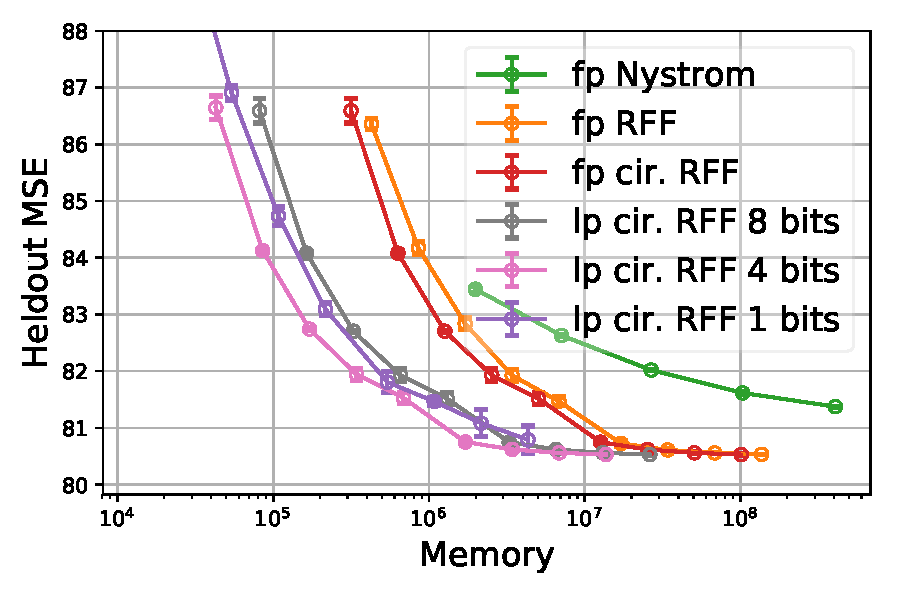
\includegraphics[width=0.3\linewidth]{figures/yearpred_MSE_vs_n_memory.pdf} &
%		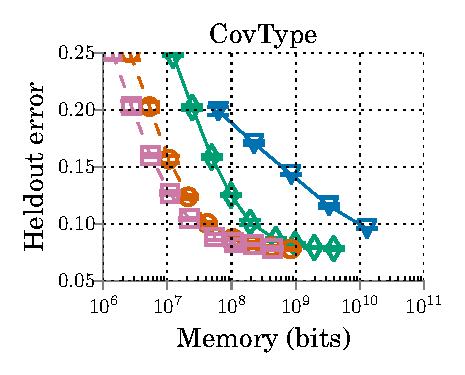
\includegraphics[width=0.3\linewidth]{figures/covtype_error_vs_n_memory.pdf} &
%		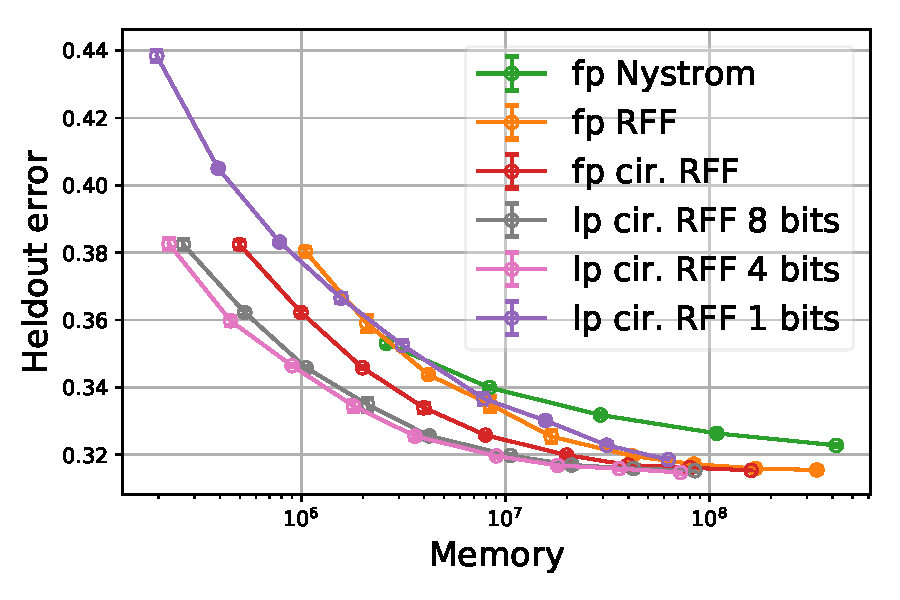
\includegraphics[width=0.3\linewidth]{figures/timit_error_vs_n_memory.pdf} \\
%		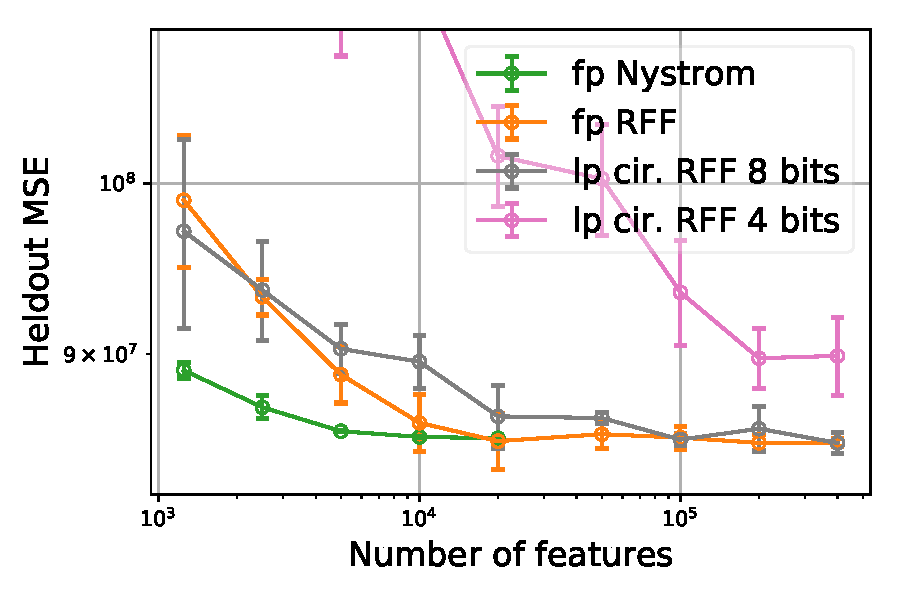
\includegraphics[width=0.3\linewidth]{figures/census_MSE_vs_n_feat.pdf} &
%		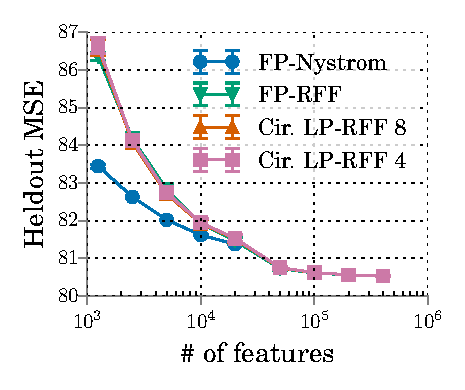
\includegraphics[width=0.3\linewidth]{figures/yearpred_MSE_vs_n_feat.pdf} &
%		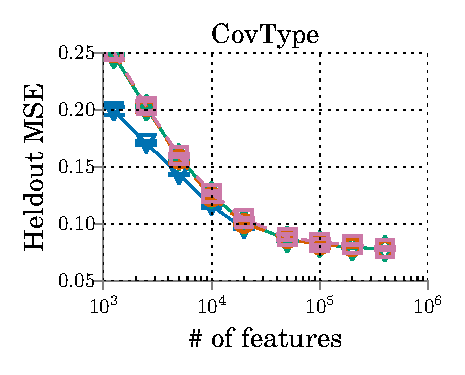
\includegraphics[width=0.3\linewidth]{figures/covtype_error_vs_n_feat.pdf} &
%		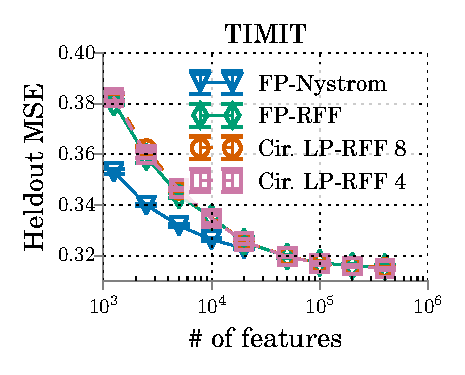
\includegraphics[width=0.3\linewidth]{figures/timit_error_vs_n_feat.pdf} \\
%		(a) Census & (b) YearPred & (c) Covtype & (d) TIMIT \\
	\end{tabular}
	\caption{Generalization performance of low precision RFF, full precision RFF and \Nystrom with respect to number of features and memory budgets. We can observe that LP RFFs demonstrate better generalization performance than full precision baselines under memory budget. Noticeably, the comparison of different methods on generalization performance behaves differently under memory budget and under number off features. E.g., \Nystrom shows better generalization performance than RFF based approach with the same number of features. However, \Nystrom can be significantly worse under memory budgets.}
	\label{fig:generalization_col_app}
\end{figure}

\begin{figure}
	\centering
	\begin{tabular}{c c c}
		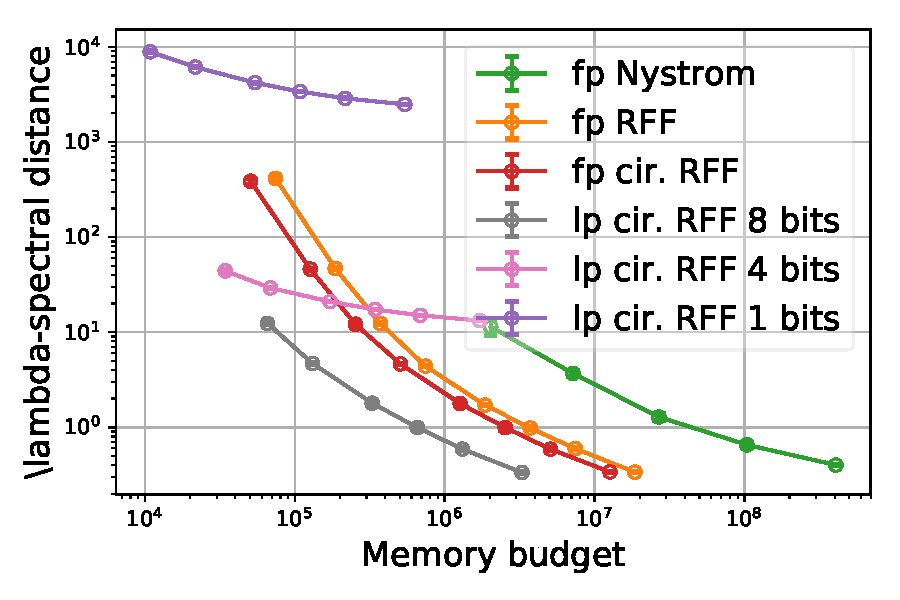
\includegraphics[width=0.33\linewidth]{figures/regression_delta_vs_mem.pdf} &
		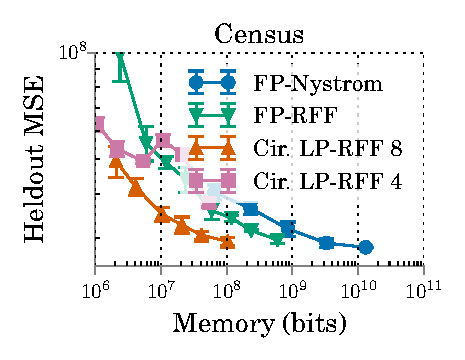
\includegraphics[width=0.33\linewidth]{figures/regression_l2_vs_mem.pdf} &
		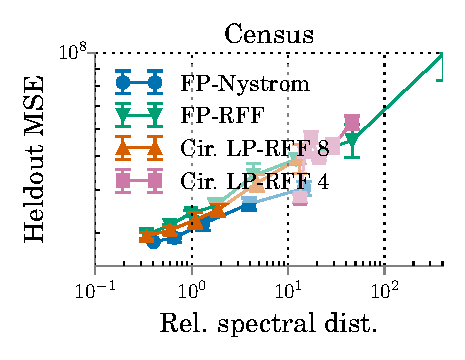
\includegraphics[width=0.33\linewidth]{figures/regression_l2_vs_delta.pdf} \\
		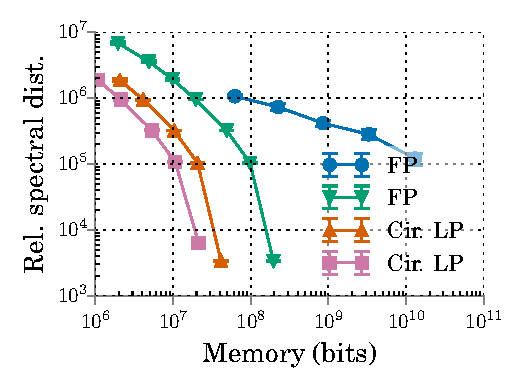
\includegraphics[width=0.33\linewidth]{figures/classification_delta_vs_mem.pdf} &
		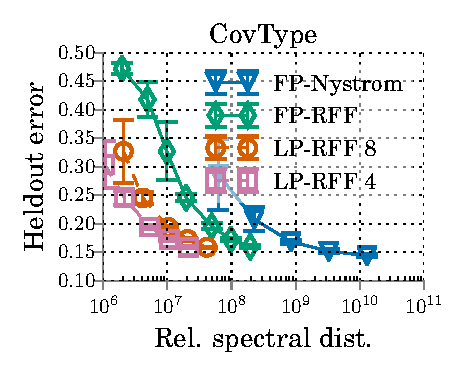
\includegraphics[width=0.33\linewidth]{figures/classification_acc_vs_mem.pdf} &
		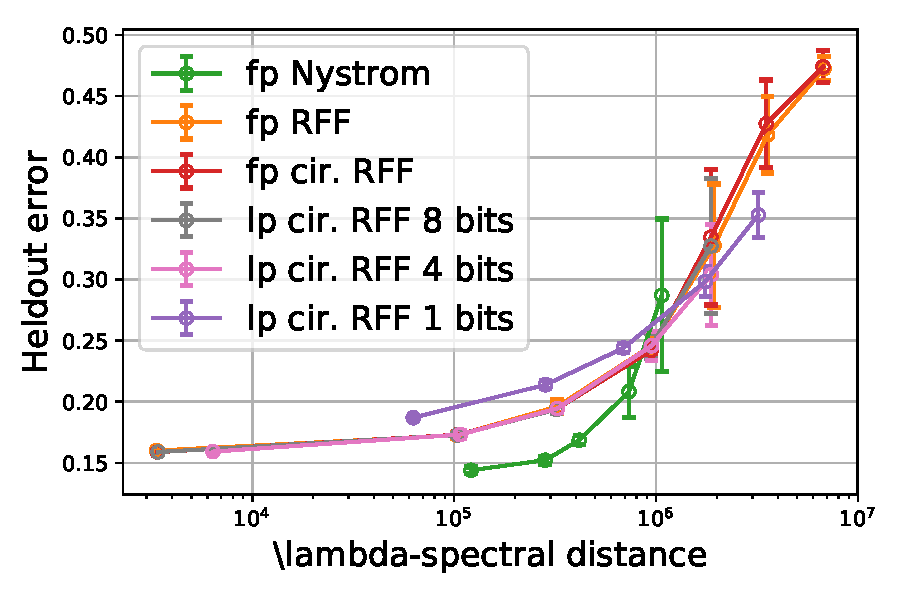
\includegraphics[width=0.33\linewidth]{figures/classification_acc_vs_delta.pdf} \\
		(a) & (b) & (c)
	\end{tabular}
	\caption{The strong correlation between generalization performance and $\lambda$-spectral distance $D_{\lambda}(K,\tK)$ under memory budgets for the Census dataset (top) and subsampled CovType dataset (bottom). Under different memory budget in (a) and (b), the precision demonstrates smaller $D_{\lambda}(K,\tK)$ tends to have better generalization performance. In (c), different kernel approximation approaches demonstrate similar generalization performance for similar $\lambda$-spectral distance.}
	\label{fig:specdist_app}
\end{figure}


